\documentclass[handout]{beamer} % [handout] para imprimir eliminando transiciones

%\usefonttheme[onlymath]{serif}
%\usepackage{fontspec}
%\defaultfontfeatures{Mapping=tex-text}
%\setsansfont[Ligatures={Common}]{Futura}
%\setmonofont[Scale=0.8]{Monaco} 

\usepackage{beamerthemesplit}
\usepackage[utf8]{inputenc}
\usepackage[spanish]{babel}
\mode<presentation>
\usetheme{default}
\usecolortheme{dolphin}
\usepackage{alltt}                                    % \begin{alltt}
\usepackage{amssymb}                                  % mathematical symbols
\usepackage{comment}
\usepackage{tabto}                                    % \tabto
\usepackage{tikz}
\usetikzlibrary{automata}
\usetikzlibrary{positioning}
\usetikzlibrary{calc}

\usepackage{verbatim}                                 % comentarios

\title{Lenguajes de Programación}                     %[titulo corto]
\author{Fabián Riquelme Csori}                        %[nombre corto]
\date{2017}                                           %[fecha corta]
\institute{Universidad de Valparaíso}                 %[instituto corto]

\newcommand{\HRule}{\rule{\linewidth}{0.2mm}\\[1ex]}
\newcommand{\blue}[1]{\textcolor{blue}{#1}}
\newcommand{\red}[1]{\textcolor{red}{#1}}
\newcommand{\redb}[1]{{\color{red!70!black}{#1}}}
\newcommand{\green}[1]{{\color{green!70!black}{#1}}}
\newcommand{\gray}[1]{{\color{gray!50!white}{#1}}}
\newcommand{\yell}[1]{{\color{yellow!70!black}{#1}}}
\newcommand{\lQ}{\mbox{``}}
\newcommand{\rQ}{\mbox{''}}
% \alert{texto destacado en rojo}
% \color{green} Color en verde
% \structure{texto en lila}


\begin{document}

%\begin{frame}%[plain]
%  \titlepage
%\end{frame}
%
% [opciones]:
% plain: oculta barra de navegacion, deja + espacio para contenido
% fragile: usar comandos como verbatim
% b,c,t: alineacion vertical
% label=nombre_etiqueta
% allowframebreaks: divide contenido en varios frames si es demasiado largo
% shrink: para escribir mucho texto en una transparencia, reduciendo tamano de fuente

%%%%%%%%%% PORTADA %%%%%%%%%%
\begin{frame}[plain]
  \begin{figure}[h]
    \begin{minipage}{0.3\textwidth}
    
\includegraphics[width=.9\textwidth]{./image/logo-UV.png}
    \end{minipage}
    \begin{minipage}{0.65\textwidth}
     $~$\\[3.6ex]
     \footnotesize{Escuela de Ingeniería Civil Informática}\\
     \footnotesize{Facultad de Ingeniería}
    \end{minipage}
  \end{figure}
  \begin{center}
    \vspace{1ex}
    \HRule
    \Large{Lenguajes de Programación}\\{\small Capítulo VI: Control de flujo}\\[-1ex]
    \HRule\vspace{1ex}
    \large{Fabián Riquelme Csori}\\[.5ex]\footnotesize{fabian.riquelme@uv.cl}\\[6ex] {\tiny 2017-II}\\[6ex]
  \end{center}
\end{frame}

%%%%%%%%%% INDEX %%%%%%%%%%
\begin{frame}
 \frametitle{Index}
 \scriptsize 			% reducir tamano de letra
 \tableofcontents		%[pausesections]
\end{frame}

%%%%%%%%%%% ACTUAL INDEX %%%%%%%%%%
%\AtBeginSection[] %generar indice automaticamente
%{
%\begin{frame}<beamer>%[plain]
% \frametitle{Index}
% \framesubtitle{subtitulo}
% \scriptsize
% \tableofcontents[currentsection, currentsubsection]
%\end{frame}
%}

%==============================
\section{Flujos de control}

%------------------------------
\subsection{Mecanismos de flujo de control}

\begin{frame}{Flujo de control}
  \begin{itemize}
    \item<1-> El \blue{flujo de control} es el orden en que se ejecutan o evalúan las distintas instrucciones dentro del código de un programa.
    \item<2-> El análisis explícito del flujo de control se visualiza en las \blue{estructuras de control} (if-else, for, while, etc.) propias de los \redb{lenguajes imperativos}.
    \item<3-> Por tanto, en este capítulo ya nos alejamos de los \redb{lenguajes declarativos}.
  \end{itemize}
\end{frame}

\begin{frame}{Mecanismos de flujo de control}
  \begin{itemize}
    \item Secuenciación
    \item Selección
    \item Iteración
    \item Abstracción procedural
    \item Recursión
    \item Concurrencia
    \item Excepciones
    \item No-determinismo
  \end{itemize}
\end{frame}

\begin{frame}{1. Secuenciación}
  \begin{itemize}
    \item Los statements o expresiones se ejecutan o evalúan, respectivamente, en un orden especificado.
    \begin{itemize}
        \item Usualmente arriba-abajo, izquierda-derecha.
    \end{itemize}
  \end{itemize}
  \begin{center}
    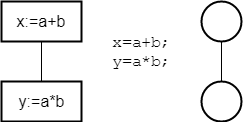
\includegraphics[width=.4\textwidth]{./image/cap6/secuenciacion}
  \end{center}
\end{frame}

\begin{frame}{2. Selección}
  \begin{itemize}
    \item<1-> Dependiendo de una condición en tiempo de ejecución, se toma una elección entre dos o más statements o expresiones.
    \item<2-> Ej: \uncover<3->{Los constructores clásicos de selección son el \blue{if-else} y el \blue{switch-case}.}
  \end{itemize}
  \uncover<3->{
  \begin{center}
    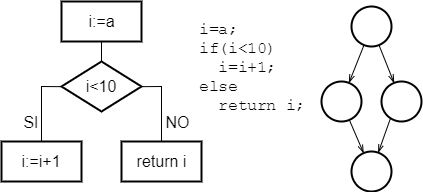
\includegraphics[width=.7\textwidth]{./image/cap6/seleccion}
  \end{center}}
  {\footnotesize \uncover<4->{¿Cómo sería un \blue{if-else-if}?}}
\end{frame}

\begin{frame}{3. Selección}
  \begin{center}
    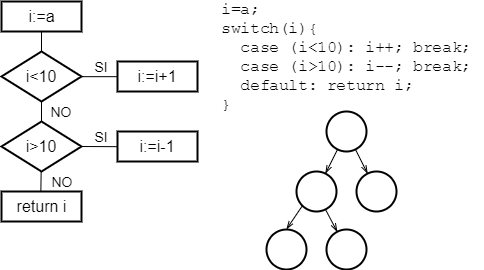
\includegraphics[width=.9\textwidth]{./image/cap6/seleccion2}
  \end{center}
\end{frame}

\begin{frame}{4. Iteración}
  \begin{itemize}
    \item<1-> Un fragmento de código se ejecuta repetidamente, ya sea una cantidad determinada de veces o hasta que se cumpla cierta condición en tiempo de ejecución.
    \item<2-> Constructos clásicos de iteración son \blue{for}, \blue{while/do-while}, \blue{repeat-until}.
  \end{itemize}
  \uncover<2->{
  \begin{center}
    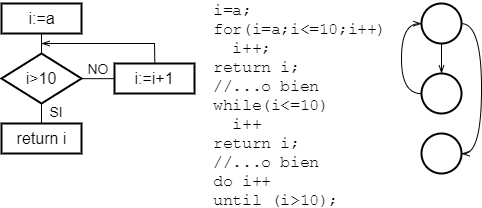
\includegraphics[width=.9\textwidth]{./image/cap6/iteracion}
  \end{center}}
\end{frame}

\begin{frame}{5. Abstracción procedural}
  \begin{itemize}
    \item Una colección potencialmente compleja de constructor de control (una función o subrutina) son encapsulados de manera de ser tratados como una única unidad, usualmente parametrizable.
  \end{itemize}
\end{frame}

\begin{frame}{6. Recursión}
  \begin{itemize}
    \item Una expresión se define en términos de (versiones más simples de) sí misma; ya sea directa o indirectamente.
    \item El modelo computacional requiere una pila en la cual almacenar información parcial de las expresiones evaluadas.
    \item Las recursiones usualmente se implementan en base a subrutinas con auto-referencias.
  \end{itemize}
\end{frame}

\begin{frame}{7. Concurrencia}
  \begin{itemize}
    \item<1-> Dos o más fragmentos de programa se ejecutan o evalúan ``al mismo tiempo'', ya sea en paralelo o en procesadores separados, o bien intercalados en un mismo procesador.
    \item<2-> No confundir \blue{concurrencia} con \blue{paralelismo}.
    \begin{itemize}
        \item<3-> Dos hebras corriendo en un computador con 1 procesador y 1 núcleo son concurrentes, pero no paralelas.
        \item<4-> El paralelismo es una abstracción pensada para mejorar el rendimiento de un proceso.
        \item<4-> La concurrencia es necesaria para implementar el paralelismo.
    \end{itemize}
  \end{itemize}
\end{frame}

\begin{frame}{8. Excepciones}
  \begin{itemize}
    \item<1-> Un fragmento de programa se ejecuta optimistamente, bajo el supuesto de que alguna condición esperada sera cierta.
    \item<1-> Si la condición resulta falsa, la ejecución se redirige hacia un \blue{handler} (manejador de excepciones) que reemplaza el resto de la ejecución.
    \item<2-> Ej. en Python:\\[1.5ex]
{\footnotesize
\texttt{try:}\\
\texttt{$~~~$ result = x / y}\\
\texttt{except ZeroDivisionError:}\\
\texttt{$~~~$ print "division by zero!"}\\
\texttt{else:}\\
\texttt{$~~~$ print \char`\"result is", result}\\
\texttt{finally:}\\
\texttt{$~~~$ print \char`\"executing finally clause"}}
  \end{itemize}
\end{frame}

\begin{frame}{9. No-determinismo}
  \begin{itemize}
    \item<1-> El orden o elección entre statements y expresiones es deliberadamente no especificado. Esto implica que cualquier alternativa llevará a un resultado correcto.
    \begin{itemize}
        \item Ej: variables aleatorias, \texttt{time()}...
    \end{itemize}
    \item<1-> Algunos lenguajes requieren que las opciones sean aleatorias, o bien ``justas''.
  \end{itemize}
\end{frame}

\begin{frame}{En resumen...}
  \begin{itemize}
    \item Pensar en estos mecanismos de flujo de control de manera general, más que en la sintáxis particular de un lenguaje, facilita el aprendizaje de la programación o de nuevos lenguajes.
    \item Profundizaremos en la abstracción procedural, excepciones y concurrencia unos capítulos más adelante.
    \item Lo siguiente tocará los mecanismos de secuenciación, selección, iteración y recursión.
  \end{itemize}
\end{frame}

%==============================
\section{Evaluación de expresiones}

\begin{frame}{Expresiones, operadores y funciones}
  \begin{itemize}
    \item Una \blue{expresión} es un objeto o valor simple:
    \begin{itemize}
        \item una constante literal, un identificador o variable, o bien
        \item un \redb{operador} (o función) aplicada a una colección de \redb{operandos} (o argumentos), donde cada operando o argumento es a su vez una expresión.
    \end{itemize}
    \item El término \blue{operador} se suele reservar para funciones predefinidas del lenguaje, mientras que una \blue{función} es una abstracción definida por el programador.
  \end{itemize}
\end{frame}

\begin{frame}{Azúcar sintáctico}
  \begin{itemize}
    \item<1-> El \blue{azúcar sintáctico} o {\em syntactic sugar} son decisiones sintácticas que se toman al crear un lenguaje para facilitar la lectura de operaciones.
    \item<2-> Algunos ejemplos:
    \begin{itemize}
        \item<3-> \redb{\texttt{a += b}} y \redb{\texttt{a++}} en C.
        \item<4-> \redb{\texttt{a[i]}} para decir \redb{\texttt{*(a + i)}} en C.
        \item<4-> \redb{\texttt{a->x}} para decir \redb{\texttt{(*a).x}} en C.
        \item<5-> \redb{\texttt{MOVE A TO B}} para decir \redb{\texttt{MOVE A B}} en COBOL.
        \item<5-> \redb{\texttt{a m b}} para decir \redb{\texttt{a.m(b)}} en Scala, donde \redb{\texttt{m}} es cualquier método, etc.
    \end{itemize}
  \end{itemize}
\end{frame}

\begin{frame}{Notación pre/in/post fija}
  \begin{itemize}
    \item Los lenguajes especifican un orden de precedencia para sus llamadas a función/operadores.
    \begin{itemize}
        \item Prefija: $~$\texttt{op a b} $~~~$ \texttt{op(a, b)} $~~~$ \texttt{(op a b)}
        \item Infija: $~~$ \texttt{a op b}
        \item Posfija: $~$\texttt{a b op}
    \end{itemize}
    \item La mayoría de los lenguajes imperativos usa notación infija para los operadores con dos argumentos, y notación prefija, con paréntesis para los argumentos, para otras funciones.
    \item Lenguajes funcionales como Lisp, Scheme y Racket usan notación postfija, tipo \texttt{(op a b)}, para todas las aplicaciones de funciones y operadores.
  \end{itemize}
\end{frame}

\begin{frame}{Notación pre/in/post fija}
  \begin{itemize}
    \item<1-> Algunos lenguajes, como ML, Haskell, Scala, R, permiten crear nuevos operadores infijos.
    \item<2-> Otros lenguajes como C++, permiten sobrecargar operadores existentes.
    \item<3-> Otros lenguajes, como Smalltalk u Objective-C, definen su propia notación:
    \begin{itemize}
        \item Rectangle origin: 0 corner: 100
        \item $[$Rectangle origin:0 corner: 100$]$
    \end{itemize}
  \end{itemize}
\end{frame}

\begin{frame}{Asignaciones}
  \begin{itemize}
    \item Un elemento de un lenguaje presenta un \blue{efecto secundario} (\blue{side-effect}) si su evaluación influencia la computación subsecuente de cualquier manera distinta a retornar un valor a su contexto.
    \item Por lo tanto, una asignación de variables es un escenario principal de efectos secundarios.
    \begin{itemize}
        \item Lo que busca es cambiar el valor de una variable, influenciando el resto de la computación en la cual dicha variable aparece.
    \end{itemize}
  \end{itemize}
\end{frame}

\begin{frame}{Statements}
  \begin{itemize}
    \item<1-> Muchos lenguajes imperativos distinguen entre \blue{expresiones}, que siempre producen un valor y  pueden o no tener efectos secundarios, y los \blue{statements}, que solo se ejecutan por sus efectos secundarios.
    \item<2-> Ej: \uncover<3->{un \texttt{print}.}
    \item<4-> Los lenguajes puramente funcionales no tienen efectos secundarios. El valor de una expresión depende de su ambiente en que es evaluada, y no del momento en que se ejecuta (\blue{transparencia referencial}).
    \item<5-> Sin embargo, la mayoría de lenguajes no son 100\% puros.\\Ej: SML tiene \redb{referencias} y I/O...
  \end{itemize}
\end{frame}

\begin{frame}{Valores y Referencias}
  \begin{itemize}
    \item Hay dos modelos para implementar asignaciones:
    \begin{itemize}
        \item El \blue{modelo de valores} (Ej: C)
        \item El \blue{modelo de referencias} (Ej: SML)
    \end{itemize}
  \end{itemize}
\end{frame}

\begin{frame}{Modelo de valores}
    \begin{minipage}{0.3\textwidth}
    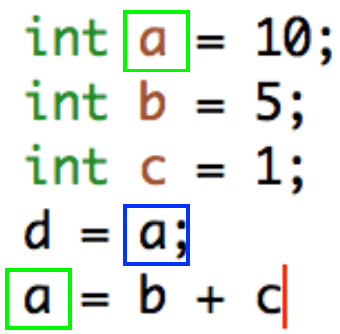
\includegraphics[width=\textwidth]{./image/cap6/valores-C}
    \end{minipage}
    \begin{minipage}{0.65\textwidth}
     \begin{itemize}
         \item \blue{l-value}: Al estar al lado izquierdo de la asignación, asignamos un nuevo valor a la dirección de memoria asociada al nombre \texttt{a}.
         \item \blue{r-value}: al estar al lado derecho de la asignación, se usa el valor almacenado en la dirección de memoria asociada al nombre \texttt{a}.
     \end{itemize}
    \end{minipage}
    \pause
    \begin{itemize}
        \item No todas las expresiones pueden ser l-values. Ej: constantes.
        \item Expresiones más complejas, como referencias obtenidas de una estructura de datos, sí pueden usarse como l-values. Es decir, no están restringidos sólo a nombres de variable.
        \item C permite combinar el modelo de valores con el modelo de referencias mediante los punteros.
    \end{itemize}
\end{frame}

\begin{frame}{Modelo de referencias}
    \begin{minipage}{0.3\textwidth}
    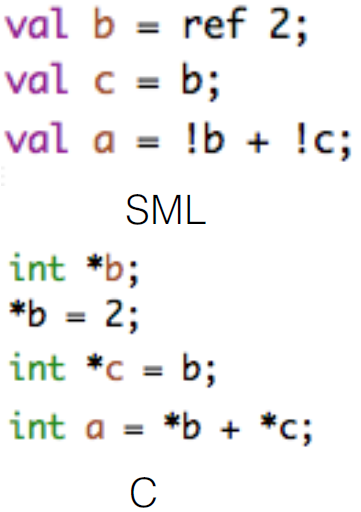
\includegraphics[width=\textwidth]{./image/cap6/valores-SML-C}
    \end{minipage}
    \begin{minipage}{0.65\textwidth}
     \begin{itemize}
         \item Una \blue{referencia} representa una \blue{indirección} hacia una ubicación de memoria que almacena un valor.
         \item Ej: punteros en C, SML.
         \item<2-> ¿Qué pasa si se actualiza el valor de b?
         \item<3-> En el modelo de referencias, toda variable es un l-value. Cuando aparece en un contexto en que necesitamos un r-value, debemos \blue{desreferenciar} la referencia para obtener el valor. En SML esto se realiza usando el operador ! (en C se usa el operador $*$).
     \end{itemize}
    \end{minipage}
\end{frame}
    
%==============================
\section{Flujo estructurado y no-estructurado}

\begin{frame}{GOTO}
    \begin{minipage}{0.3\textwidth}
    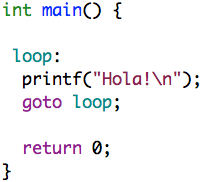
\includegraphics[width=\textwidth]{./image/cap6/goto}
    \end{minipage}
    \begin{minipage}{0.65\textwidth}
     \begin{itemize}
         \item El flujo de control en los lenguajes ensamblador se logra mediante saltos condicionales y no condicionales.
         \item Lenguajes como FORTRAN, BASIC, e incluso C, incorporan el statement \blue{goto} para realizar saltos a líneas etiquetadas.
     \end{itemize}
    \end{minipage}
\end{frame}

\begin{frame}{GOTO pecaminoso}
    \begin{itemize}
        \item<1-> En los años 1960, Dijkstra y otros detractores de la programación no estructurada provocaron que se abandonara el uso de goto (salvo por razones de compatibilidad), e introdujeron lo que hoy se conoce como \blue{programación estructurada}.
        \item<2-> La programación estructurada enfatiza el \redb{diseño top-down}, la \redb{modularización} del código, el uso de \redb{tipos estructurados}, y otras ``buenas prácticas'' que son casi innatas hoy en día.
    \end{itemize}
\end{frame}

\begin{frame}{GOTO pecaminoso}
    \begin{itemize}
        \item<1-> Los diseñadores de la programación estructurada demostraron que casi cualquier algoritmo imperativo ``bien diseñado'', puede expresarse usando secuenciación, selección e iteración.
        \item<2-> En vez de usar etiquetas, los lenguajes estructurados utilizan las fronteras de constructos con scope léxico para manipular el flujo de control.
        \item<3-> La mayoría de los constructor de flujo de control familiares para los programadores ``modernos'', tales como if-then-else, for, while, y switch, fueron desarrollados como parte de la programación estructurada.
    \end{itemize}
\end{frame}

%------------------------------

\begin{frame}
 \begin{block}{Bibliografía}
  \begin{itemize}
    \item Pratt, Terrence W. (1998). \textit{Lenguajes de programación: diseño e implementación}, Pearson Education.
    \item Sethi, Ravi (1992). \textit{Lenguajes de programación: conceptos y constructores}, Addison-Wesley Iberoamericana.
    \item Scott, Michael (2009). \textit{Programming Language Pragmatics}, Morgan Kaufman, 3ra ed.
  \end{itemize}
 \end{block}
 \begin{block}{Recursos}
  \begin{itemize}
    \item Wikipedia y Wikimedia Commons.
    \item Imágenes con licencia libre.
  \end{itemize}
 \end{block}
\end{frame}

\end{document}
